\begin{frame}
\frametitle{Summary}
\begin{block}{Monads, Comonads, Applicative Functors \ldots}
All just the names of common interfaces.
\begin{itemize}
\item with many distinct and disparate instances.
\item with many derived operations.
\end{itemize}
Each making different trade-offs for differences in utility.
\end{block}
\end{frame}

\begin{frame}
\frametitle{Utility}
\begin{block}{When might I use any of these interfaces?}
The same reason we already use interfaces; \emph{to abstract away code repetition}.
\end{block}
\end{frame}

\begin{frame}
\frametitle{Ubiquity}
\begin{block}{If these interfaces are so useful, why aren't they used everywhere?}
\begin{itemize}
\item expressibility
\item familiarity
\end{itemize}
\end{block}
\end{frame}

\begin{frame}
\frametitle{Type systems}
\begin{block}{Some type systems \textbf{limit expression} of abstraction.}
\begin{itemize}
\item Java
\item C\#
\item F\#
\end{itemize}
\end{block}
\end{frame}

\begin{frame}
\frametitle{Type systems}
\begin{center}
These type systems are limited in the kinds of interfaces that they can describe.
\end{center}
\begin{center}
The missing type system feature is called \emph{higher-kinded polymorphism}.
\end{center}
\end{frame}

\begin{frame}
\frametitle{Type systems}
\begin{block}{Some type systems render abstraction \textbf{humanly intractable}}\footnote{though some brave souls have tried}
\begin{itemize}
\item JavaScript
\item Ruby
\item Python
\end{itemize}
\end{block}
\end{frame}

\begin{frame}
\frametitle{Type systems}
\begin{center}
The likelihood of correctly utilising abstraction at the level of these interfaces approaches zero very quickly.
\end{center}
\end{frame}

\begin{frame}
\frametitle{The Parable of the listreverse project}
\begin{center}
Imagine, for a minute, a programming language that did not allow the programmer to generalise on list element types \ldots
\end{center}
\end{frame}

\begin{frame}
\frametitle{The Parable of the listreverse project}
\begin{center}
\ldots and if you wanted to reverse a list of bananas, you would solve that problem specific to bananas. 
\end{center}
\end{frame}

\begin{frame}[fragile]
\frametitle{The Parable of the listreverse project}
\begin{itemize}
\item<1-> But what if we then had to also reverse a list of oranges?
\item<2-> Well, we would copy and paste the previous code :)
\end{itemize}
\end{frame}

\begin{frame}
\frametitle{The Parable of the listreverse project}
Soon enough, there would be a listreverse project and contributors, with all the different list reversals.
\vfill
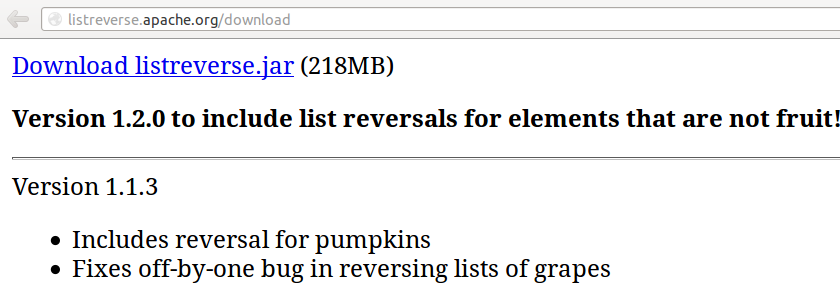
\includegraphics[height=0.3\textheight,natwidth=840,natheight=285]{image/listreverse.png}
\end{frame}

\begin{frame}
\frametitle{The Parable of the listreverse project}
\begin{block}{So, you asked\ldots}
Why don't we use a programming environment that supports reversal on \emph{any} element type?
\end{block}
\end{frame}

\begin{frame}
\frametitle{The Parable of the listreverse project}
\begin{block}{and you were told\ldots}
\begin{quote}
The listreverse project is doing just fine and is used in many enterprise projects and has many contributors successfully incorporating it into their solutions.
\end{quote}
\end{block}
\end{frame}

\begin{frame}
\frametitle{The Parable of the listreverse project}
\begin{block}{The reason}
These interfaces are not exploited is due to \emph{unfamiliarity} and tool support that discourages exploitation providing instead, the illusion of progress.
\end{block}
\end{frame}

% unfamiliarity

% lacking tool support 

% importantly, they arise regularly in all types of programming

% You do see them!

% It is my mission to help you all exploit their benefits and many more abstractions beyond.

% So please ask me more about it.